\documentclass{article}
\usepackage{tikz}
\usepackage{listings}
\usepackage{amsmath}
\usepackage[margin=1in]{geometry}

\begin{document}

\title{Binary to MIDI Conversion Algorithm}
\author{}
\date{}
\maketitle

\section{Overview}
The algorithm converts arbitrary binary data into MIDI music by interpreting bytes as musical parameters. The process involves splitting bytes into 4-bit nibbles and mapping these values to MIDI parameters.

\section{Algorithm Steps}

\subsection{1. Data Chunking}
The binary file is read in chunks, where each byte is split into two 4-bit nibbles.

\begin{center}
    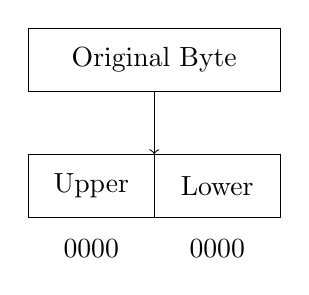
\begin{tikzpicture}[scale=0.8]
        % Original byte
        \draw (0,0) rectangle (4,1);
        \node at (2,0.5) {Original Byte};
        
        % Split into nibbles
        \draw[->] (2,0) -- (2,-1);
        \draw (0,-2) rectangle (2,-1);
        \draw (2,-2) rectangle (4,-1);
        \node at (1,-1.5) {Upper};
        \node at (3,-1.5) {Lower};
        
        % Binary representation
        \node at (1,-2.5) {0000};
        \node at (3,-2.5) {0000};
    \end{tikzpicture}
\end{center}
    
\subsection{2. MIDI Message Construction}
Each group of 8 nibbles is used to construct a MIDI message. The nibbles are allocated as follows:

\begin{itemize}
    \item Nibble 1: Channel number
    \item Nibbles 2-3: Note number
    \item Nibbles 4-5: Velocity
    \item Nibbles 6-7: Note-on timing
    \item Nibble 8: Note length
\end{itemize}

\begin{center}
    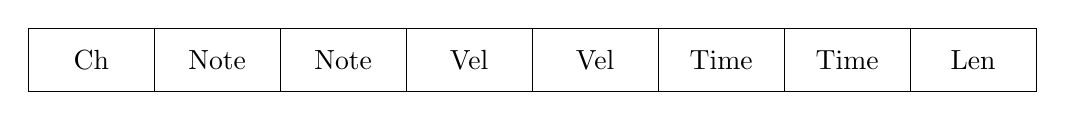
\begin{tikzpicture}[scale=0.8]
        % 8 nibbles
        \foreach \x in {0,1,...,7} {
            \draw (\x*2,0) rectangle (\x*2+2,1);
        }
        
        % Labels
        \node at (1,0.5) {Ch};
        \node at (3,0.5) {Note};
        \node at (5,0.5) {Note};
        \node at (7,0.5) {Vel};
        \node at (9,0.5) {Vel};
        \node at (11,0.5) {Time};
        \node at (13,0.5) {Time};
        \node at (15,0.5) {Len};
    \end{tikzpicture}
\end{center}

\subsection{3. Timing Calculation}
The timing information is calculated using two components:
\begin{itemize}
    \item Note-on time: Derived from two nibbles
    \item Note length: Mapped from one nibble to musical durations
\end{itemize}

\subsection{4. MIDI File Creation}
The algorithm creates two MIDI messages for each chunk:
\begin{itemize}
    \item Note-on message: Initiates the note
    \item Note-off message: Terminates the note after the calculated duration
\end{itemize}

\section{Bit Manipulation}
The algorithm uses a custom Int4 class to handle 4-bit integers.

\end{document}